\documentclass[10pt,twocolumn,letterpaper]{article}

\usepackage{cvpr}
\usepackage{times}
\usepackage{epsfig}
\usepackage{graphicx}
\usepackage{amsmath}
\usepackage{amssymb}
\usepackage{caption}
\usepackage{subcaption}
\usepackage{url}
\graphicspath{{./images/helper/}{./images/apple2orange/}{./images/summer2winter/}}

\newcommand{\norm}[1]{\left\lVert#1\right\rVert}
\newcommand{\normm}[1]{\left\lVert\lVert#1\right\rVert\rVert}

% Include other packages here, before hyperref.

% If you comment hyperref and then uncomment it, you should delete
% egpaper.aux before re-running latex.  (Or just hit 'q' on the first latex
% run, let it finish, and you should be clear).
\usepackage[breaklinks=true,bookmarks=false]{hyperref}

\cvprfinalcopy % *** Uncomment this line for the final submission

\def\cvprPaperID{****} % *** Enter the CVPR Paper ID here
\def\httilde{\mbox{\tt\raisebox{-.5ex}{\symbol{126}}}}

% Pages are numbered in submission mode, and unnumbered in camera-ready
%\ifcvprfinal\pagestyle{empty}\fi
\setcounter{page}{4321}
\begin{document}

%%%%%%%%% TITLE
\title{Exploring CycleGAN and Its Application to Font Transfer}

\author{Asif Iqbal\\
Ryerson University\\
Toronto, ON, Canada\\
{\tt\small asif1.iqbal@ryerson.ca}
% For a paper whose authors are all at the same institution,
% omit the following lines up until the closing ``}''.
% Additional authors and addresses can be added with ``\and'',
% just like the second author.
% To save space, use either the email address or home page, not both
%\and
%Second Author\\
%Institution2\\
%First line of institution2 address\\
%{\tt\small secondauthor@i2.org}
}

\maketitle
%\thispagestyle{empty}

%%%%%%%%% ABSTRACT
\begin{abstract}
   Unpaired image to image translation has gained quite a bit of attention with the advent of Cycle-Consistent Generative Adversarial Networks (CycleGANs). Translation domains like $horse \leftrightarrow zebra$, $apple \leftrightarrow orange$, $photo \leftrightarrow painting$, $summer \leftrightarrow winter$ and several others have been explored in the original work. In this paper, we plan to regenerate some of the works done in CycleGAN, try out a couple of the already tried domains on our own, and finally apply the CycleGAN concept to font style transfer. Specifically, we try it out on Arial to Times New Roman black fonts for single uppercase characters and also on lowercase multi-character words, and demonstrate that it might be a promising direction. Although it is not at all hard to get paired data for text fonts, we hope that our approach can in the future be extended to font image transfer tasks where paired data might indeed be hard to attain. The code has been made open source in the Github repository \href{https://github.com/asif31iqbal/cycle-gan-pytorch}{https://github.com/asif31iqbal/cycle-gan-pytorch}.
\end{abstract}

%%%%%%%%% BODY TEXT
\section{Introduction}
Image-to-image translation is a class of vision and graphics problems where the goal 
is to learn the mapping between an input image and an output image using a training 
set of aligned image pairs \cite{cyclegan}. Image to image \cite{cyclegan}. The field 
of image-to-image translation has been studied to quite an extent over the last couple 
of years. This problem can be more broadly described as converting an image from 
one representation of a given scene, $x$, to another, $y$, e.g., grayscale to color, 
image to semantic labels, edge-map to photograph \cite{pix2pix, cyclegan}. Years 
of research in computer vision, image processing, computational photography, 
and graphics have produced powerful translation systems in the supervised setting, 
where example image pairs $\{x_i , y_i\}_{i=1}^N$ are available \cite{rel1, rel2, rel3, 
rel4, rel5, rel6, rel7, rel8, rel9, rel10}. However, obtaining paired data for many 
tasks can be difficult and expensive. Obtaining input-output pairs for graphics 
tasks like artistic stylization can be even more difficult since the desired output 
is highly complex, typically requiring artistic authoring \cite{cyclegan}. Let's say 
we want to transfer a particular summer scene into a winter one and vice versa. 
We can easily imagine how the corresponding winter version of a summer scene 
or a summer version of a winter scene might look like even though we might have 
never seen a summer and winter version of the same scene side by side. Based on 
this insight, the authors of CycleGAN \cite{cyclegan} came up with the algorithm 
that can learn to translate between domains without paired input-output examples, 
assuming that there is some underlying relationship between the domains – for 
example, that they are two different renderings of the same underlying scene – and seek to learn that relationship. Although the algorithm lacks supervision in the form 
of paired examples, it can exploit supervision at the level of sets: we are given one 
set of images in domain $X$ and a different set in domain $Y$. We may train a mapping 
$G : X \leftarrow Y$ such that the output $\hat{y} = G(x)$, $x \in X$, is indistinguishable from 
images $y \in Y$ by an adversary trained to classify $\hat{y}$ apart from $y$ \cite{cyclegan}. However,
as discussed in \cite{cyclegan} that there could be infinitely many mappings $G$ that will induce the same distribution over $\hat{y}$. Also, there is the problem of mode collapse \cite{gan1}, where all input images map to the same output image and the optimization fails to make progress.

To tackle these problems, the CycleGAN \cite{cyclegan} authors leverage the notion of \textit{cycle consistency}, in the sense that if we transfer the font style of a character from Arial to Times New Roman, and then translate it back from Times New Roman to Arial, we should get back the original character. Mathematically, if we have a translator $G : X \leftarrow Y$ and another translator $F: Y \leftarrow X$, then G and F should be inverses of each other, and both mappings should be bijections. We apply this structural assumption by training both the mapping G and F simultaneously, and adding a cycle consistency loss \cite{cycle2} that encourages $F(G(x)) \approx x$ and $G(F(y)) \approx y$.

The authors \cite{cyclegan} have applied this idea to a wide range of
applications, like collection style transfer, object transfiguration, season
transfer and photo enhancement. In this paper, we first attempt to regenerate
their work and network architecture from scratch, apply it to couple of domains 
that they have already tried out, namely season ($summer \leftrightarrow winter$) 
transfer and object style transfer ($apple \leftrightarrow orange$). Next, we apply 
it to the domain of font style transfer. We limit ourselves to just two fonts - Arial and 
Times New Roman. We try it on single uppercase black English characters and on 
lowercase black English words. Although it is not difficult to get paired data for this 
sort of font style transfers for well known fonts which are widely available, there are 
unknown fonts, text and calligraphy styles that are available in the wild for which it is 
not easy to get paired data and applying the CycleGAN concept might be a good idea. 
The attempt with known fonts in this paper is a baby step towards the possible 
applicability of unknown font style transfers using cycle consistency.

\section{Related Work}
Over the last couple of years, Generative Adversarial Networks (GANs) \cite{gan1, gan2} have achieved
quite a bit of success in image generation. The key idea behind GAN's success is the \textit{adversarial 
loss} that forces the generated image to be indistinguishable from the input image. In the CycleGAN case,
the adversarial loss has been adopted in such a way that the generated images are indistinguishable from 
the images in the target domain.

Much of the related work regarding unpaired image-to-image translation have been mentioned in the 
original paper \cite{cyclegan}. Approaches like \cite{rel3, rel6, rel11, rel12} and \textbf{Pix2Pix} work on 
paired training examples, as opposed to the unpaired training concept that CycleGAN relies on.

There has been a few works on unpaired image-to-image translation as well. Works like \cite{rel13, rel14, 
rel15} uses a weight sharing strategy between domains. Another group of work like \cite{rel16, rel17, rel18} 
encourages the input and output to share specific content features even though they may differ in style. 
Unlike these approaches, the CycleGAN concept does not rely on any task specific, predefined similarity 
measurements. It's more of a general purpose framework.

As mentioned in the original paper, the idea of cycle consistency also has quite a bit of a history. Of these 
works, \cite{rel19}, \cite{rel20} and \cite{21} are the ones that are conceptually most similar to 
CycleGANs.

Neural Style Transfer \cite{rel4, rel22, rel23} is another family of work for image to image translation, 
which synthesizes an image by combining the content of one image with the style of another image. 
Again, this is a paired training concept while CycleGAN is unpaired.

The primary focus of CycleGAN and hence also of this paper, is learning the mapping between two two image collection, rather than between two specific images, by trying to capture correspondence between higher-level appearance structures. We try to apply the same idea in case of font style transfer.

\section{Problem Formulation}

We formulate our problem in the same way the original authors \cite{cyclegan} did, where the goal is to 
learn mapping between two domains $A$ and $B$ given training samples $\{a_i\}_{i=1}^N$ where $a_i \in 
A$ and $\{b_j\}_{j=1}^M$ where $b_j \in B$. The problem formulation has been depicted broadly in Figure 
\ref{fig:problem}.

\begin{figure*}[!htb]
     \centering
     \begin{subfigure}[b]{0.4\textwidth}
         \centering
         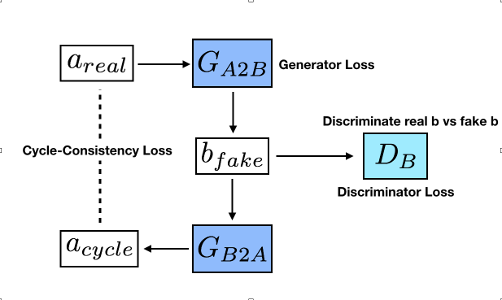
\includegraphics[width=\textwidth]{gan_b}
         \caption{Generator $G_{A2B}$ takes an image $a_{real}$ from domain $A$ and outputs $a_{fake}$ which Discriminator $D_B$ tries to distinguish from actual images in domain $B$. Image $a_{fake}$ is then passed onto generator $G_{B2A}$ which generates $a_{cycle}$. This is used for calculating the \textit{cycle-consistency} loss.}
         \label{fig:gan_b}
     \end{subfigure}
     ~
     \begin{subfigure}[b]{0.4\textwidth}
         \centering
         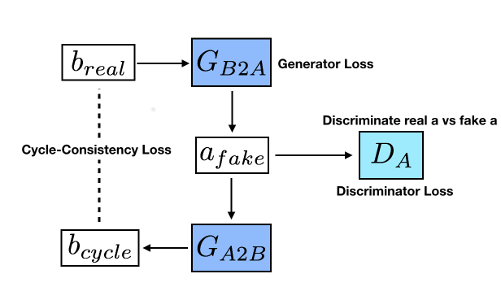
\includegraphics[width=\textwidth]{gan_a}
         \caption{Generator $G_{B2A}$ takes an image $b_{real}$ from domain $B$ and outputs $a_{fake}$ which Discriminator $D_A$ tries to distinguish from actual images in domain A. Image $b_{fake}$ is then passed onto generator $G_{A2B}$ which generates $b_{cycle}$. This is used for calculating the \textit{cycle-consistency} loss.}
         \label{fig:gan_a}
     \end{subfigure}
        \caption{Problem Formulation}
        \label{fig:problem}
\end{figure*} 

We have two generators $G_A$ and $G_B$, and two discriminators $D_A$ and $D_B$. $G_{A2B}$ takes a real 
image $a_{real}$ from domain $A$ and generates a fake image $b_{fake}$ in domain $B$, while $G_{B2A}$ 
takes a real image $b_{real}$ from domain $B$ and generates a fake image $a_{fake}$ in domain $A$. 
Discriminator $D_A$ tries to discriminate between the generated image $a_{fake}$ and real images in 
domain $A$, while discriminator $D_B$ tries to discriminate between the generated image $b_fake$ and 
real images in domain $B$. The generated fake image $b_{fake}$ is then fed back to $G_{B2A}$ to 
generate an image $a_{cycle}$ in domain $A$, while the generated fake image $a_{fake}$ is then fed back 
to $G_{A2B}$ to generate an image $b_{cycle}$ in domain $B$. 

\subsection{Loss Functions}
As can be seen from Figure \ref{fig:problem}, there are broadly 2 sorts of losses - \textit{adversarial 
loss} (generator loss and discriminator loss) and \textit{cycle-consistency loss}. The adversarial loss 
comprises of the losses incurred from the generators trying to fool the discriminators to take fake 
images as real in their corresponding domain, and from the discriminators trying to distinguish fake 
images from real ones. As discussed in \cite{cyclegan}, with large enough capacity, a network can map 
the same set of input images to any random permutation of images in
the target domain, where any of the learned mappings can
induce an output distribution that matches the target distribution.
Thus, adversarial losses alone cannot guarantee
that the learned function can map an individual input $a_{real}$
to a desired output $y_{fake}$. This is where the \textit{cycle-consistency} loss kicks in - the image 
$a_{cycle}$ should be the same as image $a_{real}$, and the image $b_{cycle}$ should be the same as 
image $b_{real}$.

To be complete, the loss functions can be broken down into the following components:

\begin{enumerate}
\item $D_A$ must approve all the original images $a_{real}$ of the domain $A$
\item $D_A$ must reject all the images $b_{fake}$ which are generated by $G_{B2A}$ to fool it
\item $G_{B2A}$ must make $D_A$ approve all the generated images $b_{fake}$, so as to fool it
\item Image $b_{cycle}$ must retain the property of original image $b_{real}$
\item $D_B$ must approve all the original images $b_{real}$ of the domain $B$
\item $D_B$ must reject all the images $a_{fake}$ which are generated by $G_{A2B}$ to fool it
\item $G_{A2B}$ must make $D_B$ approve all the generated images $a_{fake}$, so as to fool it
\item Image $a_{cycle}$ must retain the property of original image $a_{real}$
\end{enumerate}

In the above list, items $1, 2, 3, 5, 6$ and $7$ are adversarial components of the loss, while items 
$4$ and $8$ a re the \textit{cycle-consistency} components.

The original authors used $L_2$ (MSE) loss for the adversarial components, and $L_1$ loss for the 
\textit{cycle-consistency} component since it earned them better results. We adhere to the same 
principle for our work. The loss equations can be mathematically written as follows:

\begin{align*}
\begin{split}
	\mathcal{L}_{disc} ={}& \norm{D_A(a_{real}) - 1}_2 + \norm{D_B(b_{real}) - 1}_2 + \\
							   	     & \norm{D_A(a_{fake}) - 0}_2 + \norm{D_B(b_{fake}) - 0}_2\\ 
\end{split}
\end{align*}

%$\mathcal{L}_{disc} &= \norm{D_A(a_{real}) - 1}_2 + \norm{D_B(b_{real}) - 1}_2 + \\
%							   & \norm{D_A(a_{fake}) - 0}_2 + \norm{D_B(b_{real}) - 0}_2$ \\ 

This captures 1, 2, 5 and 6 above.\\

$\mathcal{L}_{gen} = \norm{D_A(a_{fake}) - 0}_2 + \norm{D_B(b_{fake}) - 0}_2$ \\

This captures 3  and 7 above.\\

$\mathcal{L}_{cycle} = \norm{a_{real} - a_{cycle}}_1  + \norm{b_{real} - b_{cycle}}_1$ \\ 

This captures 4 and 8 above.\\

So the total loss comes down to:

$\mathcal{L}_{total} = \mathcal{L}_{disc} + \mathcal{L}_{gen} + \lambda\mathcal{L}_{cycle}$\\

where $\lambda$ is a parameter to control how much weight we want to put on the \textit{cycle-consistency} as opposed to the adversarial behaviour.

\section{Data Collection}

For the $summer \leftrightarrow winter$ and $apple \leftrightarrow orange$ transformations, we collect 
the datasets from the original authors' source data \cite{data1}. The \textit{summer2winter} dataset contains 1231 train and 309 test images for summer and 962 train and 238 test images for winter. The \textit{apple2orange} dataset contains 995 train and 266 test images for apple and 1019 train and 248 test images for orange.

For the font style transfer, we have written python programs (included in the github repository) to generate images of single uppercase English characters and lowercase words. We obtain the words vocabulary from \cite{data2}. For the single uppercase character scenario, we generated 11 train images and 10 test images for each character with random scaling and translation, so in total we got 286 train images and 260 test images. For the word scenario, we randomly sampled 1981 words from \cite{data2} to create four disjoint datasets (sizes 500, 493, 496, 492) in a way that each of them has an approximately equal number of words starting with a certain character, to avoid bias as much as possible. We used the first 2 of these sets to generate images with Arial font and use those for training and testing respectively. Similarly, we used the latter 2 sets to generate training and testing images for Times New Roman font. We also applied random scaling and translation to the words before generating the words. 

\section{Network Architecture}
We essentially rebuilt the same network architecture as the original authors 
\cite{cyclegan} have used. The architecture is shown in Figure \ref{fig:architecture}. 
The numbers of channels at all intermediate stage have been shown in red, as well as 
the kernel, stride and padding size in blue. If the type of padding is Reflection 
padding, it has been used indicated in the figure in the corresponding blocks, 
otherwise padding is done with 0 values everywhere else. 

\begin{figure*}[!htb]
     \centering
     \begin{subfigure}[b]{\textwidth}
         \centering
         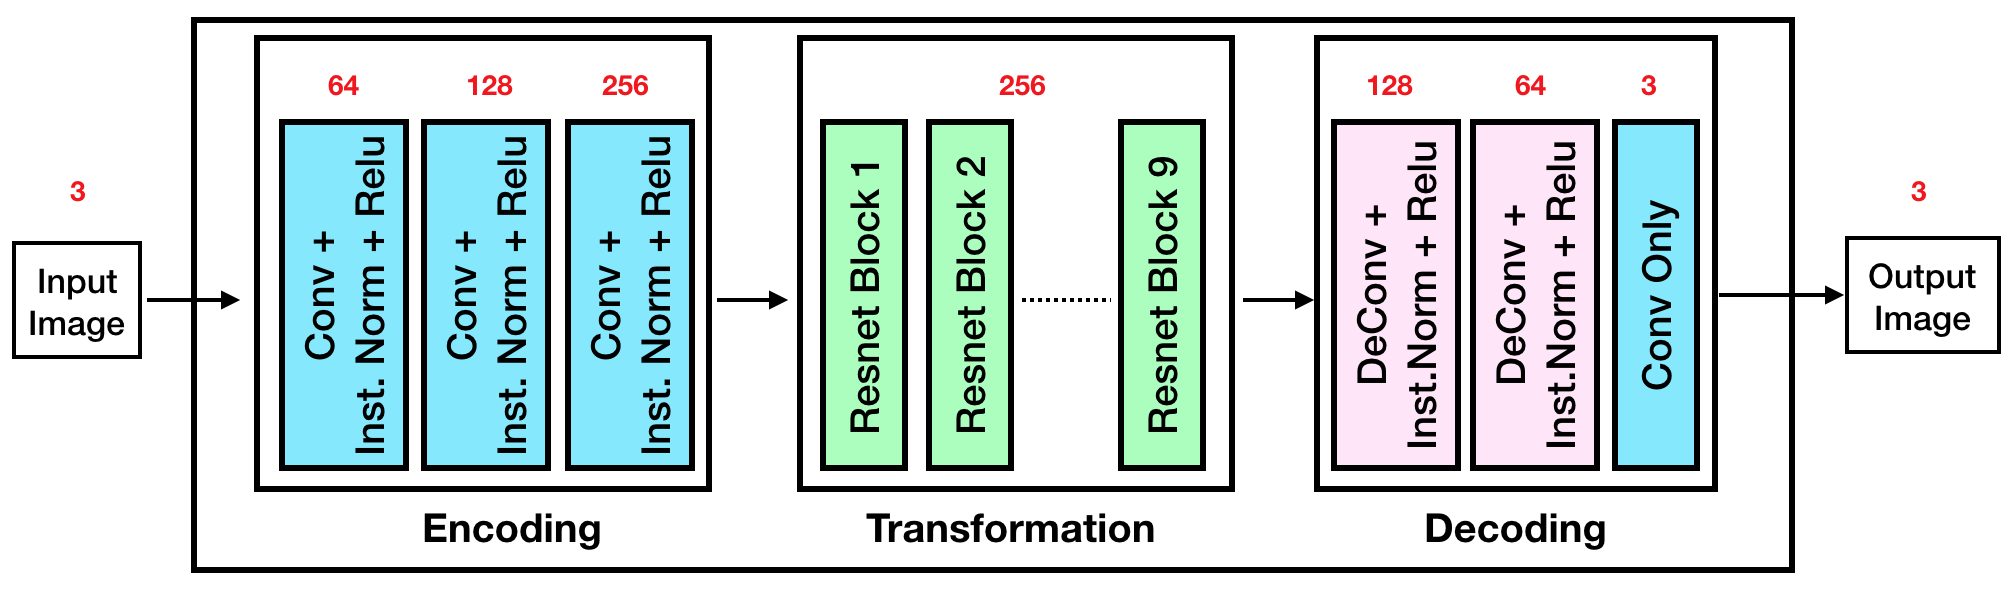
\includegraphics[width=\textwidth]{generator}
         \caption{Generator}
         \label{fig:gen}
     \end{subfigure}
     \vfill
     \begin{subfigure}[b]{0.6\textwidth}
         \centering
         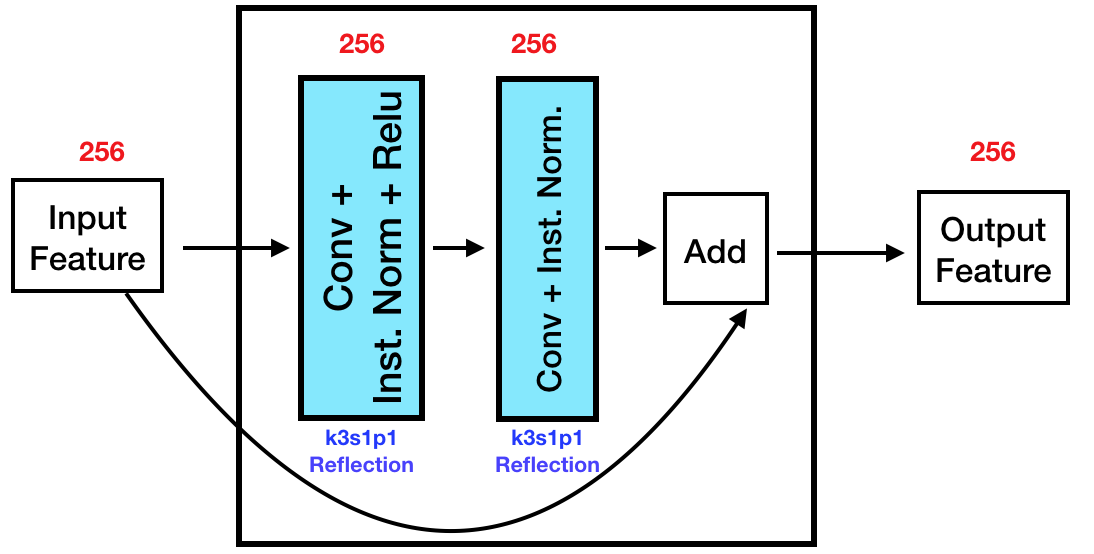
\includegraphics[width=\textwidth]{res_block}
         \caption{Resnet Block in Detail}
         \label{fig:res}
     \end{subfigure}
     \vfill
     \begin{subfigure}[b]{0.8\textwidth}
         \centering
         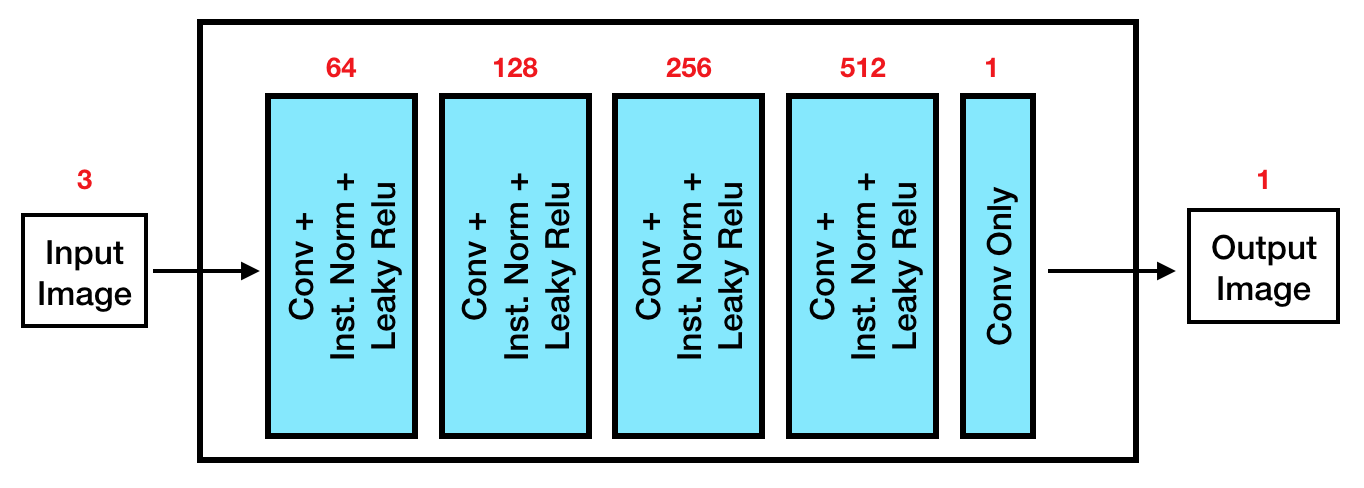
\includegraphics[width=\textwidth]{discriminator}
         \caption{Discriminator}
         \label{fig:disc}
     \end{subfigure}
        \caption{Network Architecture. The numbers in red refers to the number of output channels of each block. The letter-number combination in blue in form k\textit{x}s\textit{y}p\textit{z} beneath the blocks corresponds to the kernel size ($x$), stride ($y$) and padding ($z$). For example, k4s2p1 would mean a kernel size of $4 \times 4$, stride of 1 and padding of 1. If the padding is form $z-z$ , that means that a padding of $z$ is applied to the output as well (in addition to the input padding of $z$). The use of reflection padding has been indicated by the word Reflection in blue}
        \label{fig:architecture}
\end{figure*} 

\subsection{Generator}
The generator has 3 main segments - Encoding, Transformation an Decoding. Figure 
\ref{fig:architecture}\subref{fig:gen} The encoding part has 3 general convolutional
layers each of which is a convolution followed by instance normalization \cite{cyclegan} and Relu.b The transformation part is a series of 9 residual 
blocks (shown in more detail in Figure \ref{fig:architecture}\subref{fig:res}). Finally, the decoding segment is a couple of general deconvolutional layer followed by a convolution+tanh(kernel size 7). Each general deconvolutional layer is a deconvolution followed by instance normalization and Relu. The details have benn shown in Figure \ref{fig:architecture}\subref{fig:gen}.

\subsection{Discriminator}
For the discriminator, we use the same $70 \times 70$ PatchGAN concept used in \cite{cyclegan}.
It basically has 4 general convolutional layers. The first one is a convolution plus Leaky Relu, while the other three are convolution plus instance normalization plus Leaky Relu. These 4 layers are then followed by one single 
convolution only layer. The details have been shown in red in Figure \ref{fig:architecture}\subref{fig:disc}.

Notice that both the generator and the discriminator networks are end-to-end fully convolutional. Before 
feeding our images to these networks, we resize them to $256 \times 256$. The output size of the generator network would be of the same size as it's input ($256 \times 256 \times 3$). The output of the 
discriminator is just a one single channel $30 \times 30$ feature map, which is compared against a $30 \times 30$ all 1's or all 0's tensor while calculating discriminator loss.

\section{Experimentation}

We train our networks on a GeForce 1080 GPU using the training data collected for $summer2winter$ and $apple2orange$, and also using the generated training data for our
font style transfer.




%-------------------------------------------------------------------------
\subsection{Language}

All manuscripts must be in English.

\subsection{Dual submission}

Please refer to the author guidelines on the CVPR 2015 web page for a
discussion of the policy on dual submissions.

\subsection{Paper length}
For CVPR 2015, the rules about paper length have changed, so please
read this section carefully. Papers, excluding the references section,
must be no longer than eight pages in length. The references section
will not be included in the page count, and there is no limit on the
length of the references section. For example, a paper of eight pages
with two pages of references would have a total length of 10 pages.
{\bf Unlike previous years, there will be no extra page charges for
  CVPR 2015.}

Overlength papers will simply not be reviewed.  This includes papers
where the margins and formatting are deemed to have been significantly
altered from those laid down by this style guide.  Note that this
\LaTeX\ guide already sets figure captions and references in a smaller font.
The reason such papers will not be reviewed is that there is no provision for
supervised revisions of manuscripts.  The reviewing process cannot determine
the suitability of the paper for presentation in eight pages if it is
reviewed in eleven.  

%-------------------------------------------------------------------------
\subsection{The ruler}
The \LaTeX\ style defines a printed ruler which should be present in the
version submitted for review.  The ruler is provided in order that
reviewers may comment on particular lines in the paper without
circumlocution.  If you are preparing a document using a non-\LaTeX\
document preparation system, please arrange for an equivalent ruler to
appear on the final output pages.  The presence or absence of the ruler
should not change the appearance of any other content on the page.  The
camera ready copy should not contain a ruler. (\LaTeX\ users may uncomment
the \verb'\cvprfinalcopy' command in the document preamble.)  Reviewers:
note that the ruler measurements do not align well with lines in the paper
--- this turns out to be very difficult to do well when the paper contains
many figures and equations, and, when done, looks ugly.  Just use fractional
references (e.g.\ this line is $095.5$), although in most cases one would
expect that the approximate location will be adequate.

\subsection{Mathematics}

Please number all of your sections and displayed equations.  It is
important for readers to be able to refer to any particular equation.  Just
because you didn't refer to it in the text doesn't mean some future reader
might not need to refer to it.  It is cumbersome to have to use
circumlocutions like ``the equation second from the top of page 3 column
1''.  (Note that the ruler will not be present in the final copy, so is not
an alternative to equation numbers).  All authors will benefit from reading
Mermin's description of how to write mathematics:
\url{http://www.pamitc.org/documents/mermin.pdf}.


\subsection{Blind review}

Many authors misunderstand the concept of anonymizing for blind
review.  Blind review does not mean that one must remove
citations to one's own work---in fact it is often impossible to
review a paper unless the previous citations are known and
available.

Blind review means that you do not use the words ``my'' or ``our''
when citing previous work.  That is all.  (But see below for
techreports.)

Saying ``this builds on the work of Lucy Smith [1]'' does not say
that you are Lucy Smith; it says that you are building on her
work.  If you are Smith and Jones, do not say ``as we show in
[7]'', say ``as Smith and Jones show in [7]'' and at the end of the
paper, include reference 7 as you would any other cited work.

An example of a bad paper just asking to be rejected:
\begin{quote}
\begin{center}
    An analysis of the frobnicatable foo filter.
\end{center}

   In this paper we present a performance analysis of our
   previous paper [1], and show it to be inferior to all
   previously known methods.  Why the previous paper was
   accepted without this analysis is beyond me.

   [1] Removed for blind review
\end{quote}


An example of an acceptable paper:

\begin{quote}
\begin{center}
     An analysis of the frobnicatable foo filter.
\end{center}

   In this paper we present a performance analysis of the
   paper of Smith \etal [1], and show it to be inferior to
   all previously known methods.  Why the previous paper
   was accepted without this analysis is beyond me.

   [1] Smith, L and Jones, C. ``The frobnicatable foo
   filter, a fundamental contribution to human knowledge''.
   Nature 381(12), 1-213.
\end{quote}

If you are making a submission to another conference at the same time,
which covers similar or overlapping material, you may need to refer to that
submission in order to explain the differences, just as you would if you
had previously published related work.  In such cases, include the
anonymized parallel submission~\cite{Authors14} as additional material and
cite it as
\begin{quote}
[1] Authors. ``The frobnicatable foo filter'', F\&G 2014 Submission ID 324,
Supplied as additional material {\tt fg324.pdf}.
\end{quote}

Finally, you may feel you need to tell the reader that more details can be
found elsewhere, and refer them to a technical report.  For conference
submissions, the paper must stand on its own, and not {\em require} the
reviewer to go to a techreport for further details.  Thus, you may say in
the body of the paper ``further details may be found
in~\cite{Authors14b}''.  Then submit the techreport as additional material.
Again, you may not assume the reviewers will read this material. 

Sometimes your paper is about a problem which you tested using a tool which
is widely known to be restricted to a single institution.  For example,
let's say it's 1969, you have solved a key problem on the Apollo lander,
and you believe that the CVPR70 audience would like to hear about your
solution.  The work is a development of your celebrated 1968 paper entitled
``Zero-g frobnication: How being the only people in the world with access to
the Apollo lander source code makes us a wow at parties'', by Zeus \etal.

You can handle this paper like any other.  Don't write ``We show how to
improve our previous work [Anonymous, 1968].  This time we tested the
algorithm on a lunar lander [name of lander removed for blind review]''.
That would be silly, and would immediately identify the authors. Instead
write the following:
\begin{quotation}
\noindent
   We describe a system for zero-g frobnication.  This
   system is new because it handles the following cases:
   A, B.  Previous systems [Zeus et al. 1968] didn't
   handle case B properly.  Ours handles it by including
   a foo term in the bar integral.

   ...

   The proposed system was integrated with the Apollo
   lunar lander, and went all the way to the moon, don't
   you know.  It displayed the following behaviours
   which show how well we solved cases A and B: ...
\end{quotation}
As you can see, the above text follows standard scientific convention,
reads better than the first version, and does not explicitly name you as
the authors.  A reviewer might think it likely that the new paper was
written by Zeus \etal, but cannot make any decision based on that guess.
He or she would have to be sure that no other authors could have been
contracted to solve problem B.

FAQ: Are acknowledgements OK?  No.  Leave them for the final copy.


\begin{figure}[t]
\begin{center}
\fbox{\rule{0pt}{2in} \rule{0.9\linewidth}{0pt}}
   %\includegraphics[width=0.8\linewidth]{egfigure.eps}
\end{center}
   \caption{Example of caption.  It is set in Roman so that mathematics
   (always set in Roman: $B \sin A = A \sin B$) may be included without an
   ugly clash.}
\label{fig:long}
\label{fig:onecol}
\end{figure}

\subsection{Miscellaneous}

\noindent
Compare the following:\\
\begin{tabular}{ll}
 \verb'$conf_a$' &  $conf_a$ \\
 \verb'$\mathit{conf}_a$' & $\mathit{conf}_a$
\end{tabular}\\
See The \TeX book, p165.

The space after \eg, meaning ``for example'', should not be a
sentence-ending space. So \eg is correct, {\em e.g.} is not.  The provided
\verb'\eg' macro takes care of this.

When citing a multi-author paper, you may save space by using ``et alia'',
shortened to ``\etal'' (not ``{\em et.\ al.}'' as ``{\em et}'' is a complete word.)
However, use it only when there are three or more authors.  Thus, the
following is correct: ``
   Frobnication has been trendy lately.
   It was introduced by Alpher~\cite{Alpher02}, and subsequently developed by
   Alpher and Fotheringham-Smythe~\cite{Alpher03}, and Alpher \etal~\cite{Alpher04}.''

This is incorrect: ``... subsequently developed by Alpher \etal~\cite{Alpher03} ...''
because reference~\cite{Alpher03} has just two authors.  If you use the
\verb'\etal' macro provided, then you need not worry about double periods
when used at the end of a sentence as in Alpher \etal.

For this citation style, keep multiple citations in numerical (not
chronological) order, so prefer \cite{Alpher03,Alpher02,Authors14} to
\cite{Alpher02,Alpher03,Authors14}.


\begin{figure*}
\begin{center}
\fbox{\rule{0pt}{2in} \rule{.9\linewidth}{0pt}}
\end{center}
   \caption{Example of a short caption, which should be centered.}
\label{fig:short}
\end{figure*}

%------------------------------------------------------------------------
\section{Formatting your paper}

All text must be in a two-column format. The total allowable width of the
text area is $6\frac78$ inches (17.5 cm) wide by $8\frac78$ inches (22.54
cm) high. Columns are to be $3\frac14$ inches (8.25 cm) wide, with a
$\frac{5}{16}$ inch (0.8 cm) space between them. The main title (on the
first page) should begin 1.0 inch (2.54 cm) from the top edge of the
page. The second and following pages should begin 1.0 inch (2.54 cm) from
the top edge. On all pages, the bottom margin should be 1-1/8 inches (2.86
cm) from the bottom edge of the page for $8.5 \times 11$-inch paper; for A4
paper, approximately 1-5/8 inches (4.13 cm) from the bottom edge of the
page.

%-------------------------------------------------------------------------
\subsection{Margins and page numbering}

All printed material, including text, illustrations, and charts, must be kept
within a print area 6-7/8 inches (17.5 cm) wide by 8-7/8 inches (22.54 cm)
high.
Page numbers should be in footer with page numbers, centered and .75
inches from the bottom of the page and make it start at the correct page
number rather than the 4321 in the example.  To do this fine the line (around
line 23)
\begin{verbatim}
%\ifcvprfinal\pagestyle{empty}\fi
\setcounter{page}{4321}
\end{verbatim}
where the number 4321 is your assigned starting page.

Make sure the first page is numbered by commenting out the first page being
empty on line 46
\begin{verbatim}
%\thispagestyle{empty}
\end{verbatim}


%-------------------------------------------------------------------------
\subsection{Type-style and fonts}

Wherever Times is specified, Times Roman may also be used. If neither is
available on your word processor, please use the font closest in
appearance to Times to which you have access.

MAIN TITLE. Center the title 1-3/8 inches (3.49 cm) from the top edge of
the first page. The title should be in Times 14-point, boldface type.
Capitalize the first letter of nouns, pronouns, verbs, adjectives, and
adverbs; do not capitalize articles, coordinate conjunctions, or
prepositions (unless the title begins with such a word). Leave two blank
lines after the title.

AUTHOR NAME(s) and AFFILIATION(s) are to be centered beneath the title
and printed in Times 12-point, non-boldface type. This information is to
be followed by two blank lines.

The ABSTRACT and MAIN TEXT are to be in a two-column format.

MAIN TEXT. Type main text in 10-point Times, single-spaced. Do NOT use
double-spacing. All paragraphs should be indented 1 pica (approx. 1/6
inch or 0.422 cm). Make sure your text is fully justified---that is,
flush left and flush right. Please do not place any additional blank
lines between paragraphs.

Figure and table captions should be 9-point Roman type as in
Figures~\ref{fig:onecol} and~\ref{fig:short}.  Short captions should be centred.

\noindent Callouts should be 9-point Helvetica, non-boldface type.
Initially capitalize only the first word of section titles and first-,
second-, and third-order headings.

FIRST-ORDER HEADINGS. (For example, {\large \bf 1. Introduction})
should be Times 12-point boldface, initially capitalized, flush left,
with one blank line before, and one blank line after.

SECOND-ORDER HEADINGS. (For example, { \bf 1.1. Database elements})
should be Times 11-point boldface, initially capitalized, flush left,
with one blank line before, and one after. If you require a third-order
heading (we discourage it), use 10-point Times, boldface, initially
capitalized, flush left, preceded by one blank line, followed by a period
and your text on the same line.

%-------------------------------------------------------------------------
\subsection{Footnotes}

Please use footnotes\footnote {This is what a footnote looks like.  It
often distracts the reader from the main flow of the argument.} sparingly.
Indeed, try to avoid footnotes altogether and include necessary peripheral
observations in
the text (within parentheses, if you prefer, as in this sentence).  If you
wish to use a footnote, place it at the bottom of the column on the page on
which it is referenced. Use Times 8-point type, single-spaced.


%-------------------------------------------------------------------------
\subsection{References}

List and number all bibliographical references in 9-point Times,
single-spaced, at the end of your paper. When referenced in the text,
enclose the citation number in square brackets, for
example~\cite{Authors14}.  Where appropriate, include the name(s) of
editors of referenced books.

\begin{table}
\begin{center}
\begin{tabular}{|l|c|}
\hline
Method & Frobnability \\
\hline\hline
Theirs & Frumpy \\
Yours & Frobbly \\
Ours & Makes one's heart Frob\\
\hline
\end{tabular}
\end{center}
\caption{Results.   Ours is better.}
\end{table}

%-------------------------------------------------------------------------
\subsection{Illustrations, graphs, and photographs}

All graphics should be centered.  Please ensure that any point you wish to
make is resolvable in a printed copy of the paper.  Resize fonts in figures
to match the font in the body text, and choose line widths which render
effectively in print.  Many readers (and reviewers), even of an electronic
copy, will choose to print your paper in order to read it.  You cannot
insist that they do otherwise, and therefore must not assume that they can
zoom in to see tiny details on a graphic.

When placing figures in \LaTeX, it's almost always best to use
\verb+\includegraphics+, and to specify the  figure width as a multiple of
the line width as in the example below
{\small\begin{verbatim}
   \usepackage[dvips]{graphicx} ...
   \includegraphics[width=0.8\linewidth]
                   {myfile.eps}
\end{verbatim}
}


%-------------------------------------------------------------------------
\subsection{Color}

Please refer to the author guidelines on the CVPR 2015 web page for a discussion
of the use of color in your document.

%------------------------------------------------------------------------
\section{Final copy}

You must include your signed IEEE copyright release form when you submit
your finished paper. We MUST have this form before your paper can be
published in the proceedings.


{\small
\bibliographystyle{ieee}
\bibliography{egbib}
}

\end{document}
